\documentclass[aps,prl,amsmath,twocolumn,amssymb,superscriptaddress]{revtex4-1}
%=============================================================================
% BEGIN UNFORGIVABLE HACKS
%=============================================================================



%=============================================================================
% END UNFORGIVABLE HACKS
%=============================================================================

\usepackage{amssymb}
\usepackage{amsthm}
\usepackage{amsfonts}
\usepackage{complexity}
\usepackage{graphicx}% Include figure files
\usepackage{dcolumn}% Align table columns on decimal point
\usepackage{bm}% bold math
\usepackage{hyperref}
\usepackage{enumerate}
\usepackage{algorithm}
\usepackage{algpseudocode}
    \renewcommand{\algorithmicrequire}{\textbf{Input:}}
    \renewcommand{\algorithmicensure}{\textbf{Output:}}
    \newcommand{\inlinecomment}[1]{\Comment {\footnotesize #1} \normalsize}
    \newcommand{\linecomment}[1]{\State \(\triangleright\) {\footnotesize #1} \normalsize}
    %\renewcommand{\algorithmiccomment}[1]{\State\(\triangleright\) #1}
    
\usepackage{multirow}

\newtheorem{theorem}{Theorem}
\newtheorem{lemma}{Lemma}
\newtheorem{definition}{Definition}
\newtheorem{corollary}{Corollary}

%    Q-circuit version 2
%    Copyright (C) 2004  Steve Flammia & Bryan Eastin
%    Last modified on: 9/16/2011
%
%    This program is free software; you can redistribute it and/or modify
%    it under the terms of the GNU General Public License as published by
%    the Free Software Foundation; either version 2 of the License, or
%    (at your option) any later version.
%
%    This program is distributed in the hope that it will be useful,
%    but WITHOUT ANY WARRANTY; without even the implied warranty of
%    MERCHANTABILITY or FITNESS FOR A PARTICULAR PURPOSE.  See the
%    GNU General Public License for more details.
%
%    You should have received a copy of the GNU General Public License
%    along with this program; if not, write to the Free Software
%    Foundation, Inc., 59 Temple Place, Suite 330, Boston, MA  02111-1307  USA

% Thanks to the Xy-pic guys, Kristoffer H Rose, Ross Moore, and Daniel Müllner,
% for their help in making Qcircuit work with Xy-pic version 3.8.  
% Thanks also to Dave Clader, Andrew Childs, Rafael Possignolo, Tyson Williams,
% Sergio Boixo, Cris Moore, Jonas Anderson, and Stephan Mertens for helping us test 
% and/or develop the new version.

\usepackage[color]{xy}
\UseCrayolaColors
\xyoption{matrix}
\xyoption{frame}
\xyoption{arrow}
\xyoption{arc}

\usepackage{ifpdf}
\ifpdf
\else
\PackageWarningNoLine{Qcircuit}{Qcircuit is loading in Postscript mode.  The Xy-pic options ps and dvips will be loaded.  If you wish to use other Postscript drivers for Xy-pic, you must modify the code in Qcircuit.tex}
%    The following options load the drivers most commonly required to
%    get proper Postscript output from Xy-pic.  Should these fail to work,
%    try replacing the following two lines with some of the other options
%    given in the Xy-pic reference manual.
\xyoption{ps}
\xyoption{dvips}
\fi

% The following resets Xy-pic matrix alignment to the pre-3.8 default, as
% required by Qcircuit.
\entrymodifiers={!C\entrybox}

%\newcommand{\bra}[1]{{\left\langle{#1}\right\vert}}
%\newcommand{\ket}[1]{{\left\vert{#1}\right\rangle}}
    % Defines Dirac notation. %7/5/07 added extra braces so that the commands will work in subscripts.
\newcommand{\qw}[1][-1]{\ar @{-} [0,#1]}
\newcommand{\eqw}[1][-1]{\ar @{-} @[Red] [0,#1]}
    % Defines a wire that connects horizontally.  By default it connects to the object on the left of the current object.
    % WARNING: Wire commands must appear after the gate in any given entry.
\newcommand{\qwx}[1][-1]{\ar @{-} [#1,0]}
    % Defines a wire that connects vertically.  By default it connects to the object above the current object.
    % WARNING: Wire commands must appear after the gate in any given entry.
\newcommand{\cw}[1][-1]{\ar @{=} [0,#1]}
    % Defines a classical wire that connects horizontally.  By default it connects to the object on the left of the current object.
    % WARNING: Wire commands must appear after the gate in any given entry.
\newcommand{\cwx}[1][-1]{\ar @{=} [#1,0]}
    % Defines a classical wire that connects vertically.  By default it connects to the object above the current object.
    % WARNING: Wire commands must appear after the gate in any given entry.
\newcommand{\gate}[1]{*+<.6em>{#1} \POS ="i","i"+UR;"i"+UL **\dir{-};"i"+DL **\dir{-};"i"+DR **\dir{-};"i"+UR **\dir{-},"i" \qw}
\newcommand{\eboxgate} [1]{*+<.6em>{#1} \POS ="i","i"+UR;"i"+UL **[red]\dir{-};"i"+DL **[red]\dir{-};"i"+DR **[red]\dir{-};"i"+UR **[red]\dir{-},"i" \eqw}
\newcommand{\circgate}[1]{*+<0.6em>[o][F-]{#1} \eqw}
\newcommand{\ecircgate}[1]{*+<0.6em>[o][F-:red]{#1} \eqw}
\newcommand{\filtergt}[1]{\eboxgate{\scriptscriptstyle{#1}}}
\newcommand{\idealdec}{*+<1.2em>{\phantom{*}} \POS ="i","i"+UL;"i"+DL **[red]\dir{-};"i"+R **[red]\dir{-};"i"+UL **[red]\dir{-},"i" \eqw}

    % Boxes the argument, making a gate.
\newcommand{\meter}{*=<1.8em,1.4em>{\xy ="j","j"-<.778em,.322em>;{"j"+<.778em,-.322em> \ellipse ur,_{}},"j"-<0em,.4em>;p+<.5em,.9em> **\dir{-},"j"+<2.2em,2.2em>*{},"j"-<2.2em,2.2em>*{} \endxy} \POS ="i","i"+UR;"i"+UL **\dir{-};"i"+DL **\dir{-};"i"+DR **\dir{-};"i"+UR **\dir{-},"i" \qw}
    % Inserts a measurement meter.
    % In case you're wondering, the constants .778em and .322em specify
    % one quarter of a circle with radius 1.1em.
    % The points added at + and - <2.2em,2.2em> are there to strech the
    % canvas, ensuring that the size is unaffected by erratic spacing issues
    % with the arc.
\newcommand{\measure}[1]{*+[F-:<.9em>]{#1} \qw}
    % Inserts a measurement bubble with user defined text.
\newcommand{\measuretab}[1]{*{\xy*+<.6em>{#1}="e";"e"+UL;"e"+UR **\dir{-};"e"+DR **\dir{-};"e"+DL **\dir{-};"e"+LC-<.5em,0em> **\dir{-};"e"+UL **\dir{-} \endxy} \qw}
    % Inserts a measurement tab with user defined text.
\newcommand{\measureD}[1]{*{\xy*+=<0em,.1em>{#1}="e";"e"+UR+<0em,.25em>;"e"+UL+<-.5em,.25em> **\dir{-};"e"+DL+<-.5em,-.25em> **\dir{-};"e"+DR+<0em,-.25em> **\dir{-};{"e"+UR+<0em,.25em>\ellipse^{}};"e"+C:,+(0,1)*{} \endxy} \qw}
\newcommand{\emeasureD}[1]{*{\xy*+=<0em,.1em>{#1}="e";"e"+UR+<0em,.25em>;"e"+UL+<-.5em,.25em> **[red]\dir{-};"e"+DL+<-.5em,-.25em> **[red]\dir{-};"e"+DR+<0em,-.25em> **[red]\dir{-};{"e"+UR+<0em,.25em>\ellipse{}};"e"+C:,+(0,1)*{} \endxy} \qw}
    % Inserts a D-shaped measurement gate with user defined text.
\newcommand{\multimeasure}[2]{*+<1em,.9em>{\hphantom{#2}} \qw \POS[0,0].[#1,0];p !C *{#2},p \drop\frm<.9em>{-}}
    % Draws a multiple qubit measurement bubble starting at the current position and spanning #1 additional gates below.
    % #2 gives the label for the gate.
    % You must use an argument of the same width as #2 in \ghost for the wires to connect properly on the lower lines.
\newcommand{\multimeasureD}[2]{*+<1em,.9em>{\hphantom{#2}} \POS [0,0]="i",[0,0].[#1,0]="e",!C *{#2},"e"+UR-<.8em,0em>;"e"+UL **\dir{-};"e"+DL **\dir{-};"e"+DR+<-.8em,0em> **\dir{-};{"e"+DR+<0em,.8em>\ellipse^{}};"e"+UR+<0em,-.8em> **\dir{-};{"e"+UR-<.8em,0em>\ellipse^{}},"i" \qw}
    % Draws a multiple qubit D-shaped measurement gate starting at the current position and spanning #1 additional gates below.
    % #2 gives the label for the gate.
    % You must use an argument of the same width as #2 in \ghost for the wires to connect properly on the lower lines.
\newcommand{\control}{*!<0em,.025em>-=-<.2em>{\bullet}}
    % Inserts an unconnected control.
\newcommand{\controlo}{*+<.01em>{\xy -<.095em>*\xycircle<.19em>{} \endxy}}
    % Inserts a unconnected control-on-0.
\newcommand{\ctrl}[1]{\control \qwx[#1] \qw}
    % Inserts a control and connects it to the object #1 wires below.
\newcommand{\ctrlo}[1]{\controlo \qwx[#1] \qw}
    % Inserts a control-on-0 and connects it to the object #1 wires below.
\newcommand{\targ}{*+<.02em,.02em>{\xy ="i","i"-<.39em,0em>;"i"+<.39em,0em> **\dir{-}, "i"-<0em,.39em>;"i"+<0em,.39em> **\dir{-},"i"*\xycircle<.4em>{} \endxy} \qw}
    % Inserts a CNOT target.
\newcommand{\qswap}{*=<0em>{\times} \qw}
    % Inserts half a swap gate.
    % Must be connected to the other swap with \qwx.
\newcommand{\multigate}[2]{*+<1em,.9em>{\hphantom{#2}} \POS [0,0]="i",[0,0].[#1,0]="e",!C *{#2},"e"+UR;"e"+UL **\dir{-};"e"+DL **\dir{-};"e"+DR **\dir{-};"e"+UR **\dir{-},"i" \qw}
    % Draws a multiple qubit gate starting at the current position and spanning #1 additional gates below.
    % #2 gives the label for the gate.
    % You must use an argument of the same width as #2 in \ghost for the wires to connect properly on the lower lines.
\newcommand{\ghost}[1]{*+<1em,.9em>{\hphantom{#1}} \qw}
    % Leaves space for \multigate on wires other than the one on which \multigate appears.  Without this command wires will cross your gate.
    % #1 should match the second argument in the corresponding \multigate.
\newcommand{\push}[1]{*{#1}}
    % Inserts #1, overriding the default that causes entries to have zero size.  This command takes the place of a gate.
    % Like a gate, it must precede any wire commands.
    % \push is useful for forcing columns apart.
    % NOTE: It might be useful to know that a gate is about 1.3 times the height of its contents.  I.e. \gate{M} is 1.3em tall.
    % WARNING: \push must appear before any wire commands and may not appear in an entry with a gate or label.
\newcommand{\gategroup}[6]{\POS"#1,#2"."#3,#2"."#1,#4"."#3,#4"!C*+<#5>\frm{#6}}
    % Constructs a box or bracket enclosing the square block spanning rows #1-#3 and columns=#2-#4.
    % The block is given a margin #5/2, so #5 should be a valid length.
    % #6 can take the following arguments -- or . or _\} or ^\} or \{ or \} or _) or ^) or ( or ) where the first two options yield dashed and
    % dotted boxes respectively, and the last eight options yield bottom, top, left, and right braces of the curly or normal variety.  See the Xy-pic reference manual for more options.
    % \gategroup can appear at the end of any gate entry, but it's good form to pick either the last entry or one of the corner gates.
    % BUG: \gategroup uses the four corner gates to determine the size of the bounding box.  Other gates may stick out of that box.  See \prop.

\newcommand{\rstick}[1]{*!L!<-.5em,0em>=<0em>{#1}}
    % Centers the left side of #1 in the cell.  Intended for lining up wire labels.  Note that non-gates have default size zero.
\newcommand{\lstick}[1]{*!R!<.5em,0em>=<0em>{#1}}
    % Centers the right side of #1 in the cell.  Intended for lining up wire labels.  Note that non-gates have default size zero.
\newcommand{\ustick}[1]{*!D!<0em,-.5em>=<0em>{#1}}
    % Centers the bottom of #1 in the cell.  Intended for lining up wire labels.  Note that non-gates have default size zero.
\newcommand{\dstick}[1]{*!U!<0em,.5em>=<0em>{#1}}
    % Centers the top of #1 in the cell.  Intended for lining up wire labels.  Note that non-gates have default size zero.
\newcommand{\Qcircuit}{\xymatrix @*=<0em>}
    % Defines \Qcircuit as an \xymatrix with entries of default size 0em.
\newcommand{\link}[2]{\ar @{-} [#1,#2]}
    % Draws a wire or connecting line to the element #1 rows down and #2 columns forward.
\newcommand{\pureghost}[1]{*+<1em,.9em>{\hphantom{#1}}}
    % Same as \ghost except it omits the wire leading to the left. 
%%%%%%%%%%%%%%%%%%%%%%%%%%%%%%%%%%%%%%%%%%%%%%%%%%%%%%%%%%%%%%%%%%%%%%%%%%%%%%%%%%%%%%%%%%
\newcommand{\multiprepareC}[2]{*+<1em,.9em>{\hphantom{#2}}\save[0,0].[#1,0];p\save !C
  *{#2},p+RU+<0em,0em>;+LU+<+.8em,0em> **\dir{-}\restore\save +RD;+RU **\dir{-}\restore\save
  +RD;+LD+<.8em,0em> **\dir{-} \restore\save +LD+<0em,.8em>;+LU-<0em,.8em> **\dir{-} \restore \POS
  !UL*!UL{\cir<.9em>{u_r}};!DL*!DL{\cir<.9em>{l_u}}\restore}
   % Draws a multiple qubit reverse-D-shaped preparation gate starting at the current position and spanning #1 additional gates below.
   % #2 gives the label for the gate.
   % You must use an argument of the same width as #2 in \pureghost for the wires to connect properly on
% the lower lines.
\newcommand{\prepareC}[1]{*{\xy*+=+<.5em>{\vphantom{#1\rule{0em}{.1em}}}*\cir{l^r};p\save*!L{#1} \restore\save+UC;+UC+<.5em,0em>*!L{\hphantom{#1}}+R **\dir{-} \restore\save+DC;+DC+<.5em,0em>*!L{\hphantom{#1}}+R **\dir{-} \restore\POS+UC+<.5em,0em>*!L{\hphantom{#1}}+R;+DC+<.5em,0em>*!L{\hphantom{#1}}+R **\dir{-} \endxy}}
   % Inserts a reverse-D-shaped preparation gate with user defined text.
\newcommand{\poloFantasmaCn}[1]{{{}^{#1}_{\phantom{#1}}}}



\def\ket#1{\left|#1\right\rangle}
\def\bra#1{\langle#1|}
\newcommand{\ketbra}[2]{|#1\rangle\!\langle#2|}
\newcommand{\braket}[2]{\langle#1|#2\rangle}
% \newcommand{\note}[1]{({\bf note: #1})}
\newcommand{\prob}[1]{{\rm Pr}\left(#1 \right)}
% \newcommand{\Tr}[1]{{\rm Tr}\!\left[#1 \right]}
\newcommand{\expect}[2]{{\mathbb{E}_{#2}}\!\left\{#1 \right\}}
\newcommand{\var}[2]{{\mathbb{V}_{#2}}\!\left\{#1 \right\}}
\newcommand{\CRej}{\text{RejF }}

\newcommand{\sinc}{\operatorname{sinc}}
\newcommand{\reset}{\mathrm{reset}}


% fix: supported only for revtex
%\newcommand{\openone}{\mathbb{I}}
% fix: unsupported with iopart
%\newcommand{\eqref}[1]{(\ref{#1})}

\newcommand{\sde}{\mathrm{sde}}
\newcommand{\Z}{\mathbb{Z}}
\newcommand{\RR}{\mathbb{R}}
\newcommand{\w}{\omega}
\newcommand{\Kap}{\kappa}

\newcommand{\Tchar}{$T$}
\newcommand{\T}{\Tchar~}
\newcommand{\TT}{\mathrm{T}}
\newcommand{\ClT}{\{{\rm Clifford}, \Tchar\}~}
\newcommand{\Tcount}{\Tchar--count~}
\newcommand{\Tcountper}{\Tchar--count}
\newcommand{\Tcounts}{\Tchar--counts~}
\newcommand{\Tdepth}{\Tchar--depth~}
\newcommand{\Zr}{\Z[i,1/\sqrt{2}]}
\newcommand{\ve}{\varepsilon}

\newcommand{\eq}[1]{\hyperref[eq:#1]{(\ref*{eq:#1})}}
\renewcommand{\sec}[1]{\hyperref[sec:#1]{Section~\ref*{sec:#1}}}
\newcommand{\app}[1]{\hyperref[app:#1]{Appendix~\ref*{app:#1}}}
\newcommand{\fig}[1]{\hyperref[fig:#1]{Figure~\ref*{fig:#1}}}
\newcommand{\thm}[1]{\hyperref[thm:#1]{Theorem~\ref*{thm:#1}}}
\newcommand{\lem}[1]{\hyperref[lem:#1]{Lemma~\ref*{lem:#1}}}
\newcommand{\tab}[1]{\hyperref[tab:#1]{Table~\ref*{tab:#1}}}
\newcommand{\cor}[1]{\hyperref[cor:#1]{Corollary~\ref*{cor:#1}}}
\newcommand{\alg}[1]{\hyperref[alg:#1]{Algorithm~\ref*{alg:#1}}}
\newcommand{\defn}[1]{\hyperref[def:#1]{Definition~\ref*{def:#1}}}


\newcommand{\targfix}{\qw {\xy {<0em,0em> \ar @{ - } +<.39em,0em>
\ar @{ - } -<.39em,0em> \ar @{ - } +
<0em,.39em> \ar @{ - }
-<0em,.39em>},<0em,0em>*{\rule{.01em}{.01em}}*+<.8em>\frm{o}
\endxy}}

\newenvironment{proofof}[1]{\begin{trivlist}\item[]{\flushleft\it
Proof of~#1.}}
{\qed\end{trivlist}}


\newcommand{\cu}[1]{{\textcolor{red}{#1}}}
\newcommand{\tout}[1]{{}}
% \newcommand{\beq}{\begin{equation}}
% \newcommand{\eeq}{\end{equation}}
% \newcommand{\beqa}{\begin{eqnarray}}
\newcommand{\good}{{\rm good}}
\newcommand{\bad}{{\rm bad}}
% \newcommand{\eeqa}{\end{eqnarray}}

\newcommand{\id}{\openone}
%\newcommand{\id}{\mathbb{I}}

\newcommand{\etal}{\emph{et al.}}
\newcommand{\ii}{\mathrm{i}}
\newcommand{\ee}{\mathrm{e}}

\hyphenation{FPGA}
\hyphenation{FPGAs}
\hyphenation{RFPE}

%%%%%%%%%%%%%%%%%%%%%%% a bit nicer hypelinks %%%%%%%%%%%%%%%%%%%%%%%%%%%%%

\usepackage[usenames,dvipsnames]{xcolor}
\hypersetup{
    colorlinks=true,       % false: boxed links; true: colored links
    linkcolor=Maroon,          % color of internal links (change box color with linkbordercolor)
    citecolor=OliveGreen,        % color of links to bibliography
    filecolor=magenta,      % color of file links
    urlcolor=Blue           % color of external links
}

%%%%%%%%%%%%%%%%%%%%%%% a bit nicer hypelinks %%%%%%%%%%%%%%%%%%%%%%%%%%%%%

\begin{document}

%=============================================================================
% FRONT MATTER
%=============================================================================

\title{Efficient Bayesian Phase Estimation}
\author{Nathan Wiebe}
\affiliation{Quantum Architectures and Computation Group, Microsoft Research, Redmond, WA (USA)}

\author{Chris Granade}
\affiliation{Centre for Engineered Quantum Systems, Sydney, NSW (Australia)}
\affiliation{School of Physics, University of Sydney, Sydney, NSW (Australia)}

\begin{abstract}
    We provide a new efficient adaptive algorithm for performing phase
    estimation that uses approximate Bayesian inference to both learn the phase and
    estimate the uncertainty in the phase directly from experimental data. Our
    method is highly flexible, recovers from failures,  can be run in the
    presence of substantial decoherence and other experimental imperfections
    and is as fast or faster than existing algorithms.
\end{abstract}

\maketitle

%=============================================================================
% \section{Introduction}
% \label{sec:intro}
%=============================================================================


Eigenvalue estimation has been a cornerstone of physics since the dawn of spectroscopy.  Quantum information theory has revolutionized our understanding of how to best learn spectral properties.
These ideas exponentially reduce the number of experiments needed to learn an eigenphase and scale optimally with the total experimental time.
This quantum approach, known as phase estimation (PE), is crucial to achieve many of the celebrated speedups promised by quantum computing~\cite{shor_polynomial-time_1995,BHM+02,ADL+05,harrow2009quantum,lanyon2010towards}.  Optimizing these algorithms is especially important for present-day experimental demonstrations of such algorithms because the number of quantum gates that can be performed is often severely limited by decoherence.

The most popular approach to PE forgoes the use of quantum resources
in favor of using classical algorithms to infer the eigenvalues of a unitary
from experimental data
\cite{Kit96,kitaev2002classical,higgins2007entanglement,SHF14,KLY15}.
Given the rapid advance of machine learning methods, this this raises the question
of whether we can speed up phase estimation or make it more robust to errors
by using modern statistical methods.

% The most popular approach to PE is known as iterative phase estimation (IPE),
% as it forgoes the use of quantum resources to infer the eigenvalues of unitary
% matrix in favor of using a classical inference algorithm to estimate the
% eigenvalues from experimental
% data~\cite{Kit96,kitaev2002classical,higgins2007entanglement,SHF14,KLY15}.  Although
% the methodologies used for inference stretch back decades,
% the ongoing revolution in machine learning has lead to a plethora of
% improved classical inference procedures, and raises an important question:
% can these ideas be used to speed up phase estimation or make it more robust to
% experimental error?

We answer this in the affirmative by providing an efficient classical inference
method, inspired by recent work on particle filtering, that is tailored
to phase estimation. Our method not only provides performance
advantages over iterative methods~\cite{Kit96,kitaev2002classical}, but
is also robust to experimental imperfections such as depolarizing noise and
small systematic errors.
This allows PE to inherit the speed and robustness of adaptive Bayesian approaches while
retaining the computational efficiency of traditional iterative methods.

In particular, iterative PE infers the eigenvalue of a given eigenvector of a unitary matrix
$U$ from a set of experiments that are performed on the circuit
\begin{equation*}
    \Qcircuit @C=1em @R=1em {
        \lstick{\ket{0}}    & \gate{H}  & \gate{Z(-M \theta)}   & \ctrl{1}   & \gate{H} & \meter & \cw \\
        \lstick{\ket{\phi}} & {/} \qw   & \qw                   & \gate{U^M} & \qw      & \qw    & \qw
    }
\end{equation*}
where $U\ket{\phi} = \ee^{\ii\phi}\ket{\phi}$ for an unknown eigenphase $\phi \in \mathbb{R}$,
and where $Z(M \theta) = \ee^{\ii M \theta Z}$ is a rotation that can be used to compare the eigenphase of $U$ to
a known reference value.
Most PE algorithms use this circuit to infer the bits
in a binary expansion of $\phi$.  The process can be made near optimal (up to $\log^*$ factors~\cite{SHF14}) and
affords an efficient inference method for these bits.

In general, the input state need not be an eigenstate of $U$.  Even if the state is a maximally mixed state then the iterative process will eventually project it into
a (possibly degenerate) eigenspace of the unitary~\cite{kitaev2002classical}.  In order to simplify the following exposition, we will assume that the input state is an eigenstate of $U$ but it can also be taken
to be a maximally mixed state without loss of generality.  We will discuss this issue further below.

%=============================================================================
% \section{Bayesian Phase Estimation}
% \label{sec:bayesian-phase-est}
%=============================================================================


Bayesian phase estimation, as introduced by Svore \etal~\cite{SHF14}, involves performing a 
set of experiments and then updating the prior distribution using Bayes' rule.
For example, if an experiment is performed with using $M$ repetitions of $U$,
$Z(M \theta)$ and a measurement outcome $E\in \{0,1\}$ is observed then Bayes'
rule states that the \emph{posterior probability} distribution for $\phi$
after observing the datum is
\begin{equation}
P(\phi|E;\theta,M) = \frac{P(E|\phi;\theta,M)P(\phi)}{\int P(E|\phi;\theta,M)P(\phi)\mathrm{d}{\phi}}.\label{eq:update}
\end{equation}
The final ingredient that is needed to perform an update is the likelihood
function $P(0|\phi;\theta,M)$. For phase estimation,
\begin{gather}
    \label{eq:likenodecohere}
    \begin{aligned}
        P(0|\phi;\theta,M) & = \frac{1+\cos(M[\phi +\theta])}{2}.
    \end{aligned}
\end{gather}
The likelihood of measuring $1$ is $1-P(0|\phi;\theta,M)$.
After using~\eq{update} to update the posterior distribution we then set the prior distribution to equal the posterior distribution.  This process is then repeated for each of the random experiments in the data set.

Bayesian inference returns a posterior
distribution over the phase, the mean and standard deviation which
provide estimates of the true eigenvalue and the algorithm's
uncertainty in that value~\cite{granade_robust_2012,ferrie_high_2014}. Estimates of
the uncertainty are not just valuable for quantifying error: they also allow us to design highly informative experiments 
 and allow the protocol to be terminated when a threshold accuracy has been reached.

\begin{figure}[t!]
    \begin{centering}
        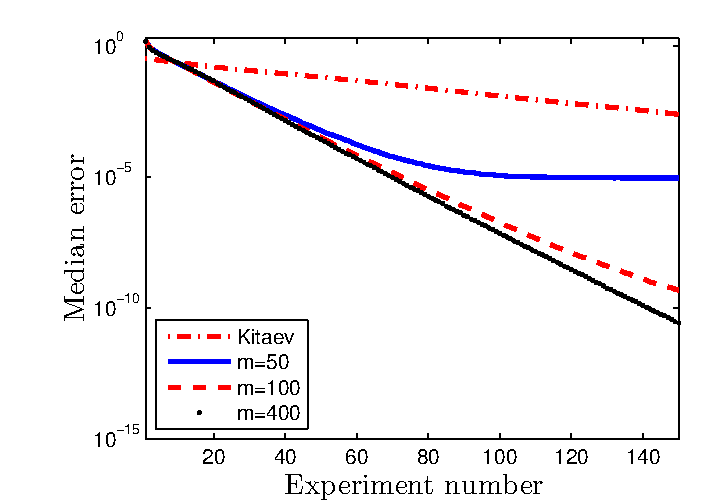
\includegraphics[width=0.8\linewidth]{PEerror.pdf}
    \end{centering}
    \caption{\label{fig:PEerror}
     Median errors in phase estimation for 10~000 random initial choices of the true eigenphase.
    }
\end{figure}




%=============================================================================
% \section{Approximate Bayesian Phase Estimation}
%=============================================================================

Exact Bayesian inference is impossible if the eigenphases are
continuous, so approximations are needed to
make the procedure tractable.  Rather than na\"ively discritizing the prior
distribution, modern methods discretize by sampling from the prior and
then perform Bayesian inference on the discrete set of samples (often called
``particles'').  These particle filter methods methods are powerful and
have become a mainstay in computer vision and machine
learning~\cite{haykin2004kalman,smith2013sequential,isard_condensationconditional_1998}.
Despite the power of particle filtering, it is often challenging to deploy in memory-limited environments,
such as on an embedded controller because thousands of particles need to be stored. With the prevalence of FPGAs in the control of
quantum information experiments
\cite{shulman_suppressing_2014,casagrande_design_2014,hornibrook_cryogenic_2015},
overcoming this limitation presents a significant advantage.

We propose a much simpler approach that we call Rejection Filtering Phase
Estimation (RFPE). RFPE works by positing a prior model and directly updates it
to find a model for our posterior, rather than using a set of hypotheses that implicitly
define a model for the system.  It achieves this by using a
Gaussian with mean $\mu$ and variance $\sigma^2$ to model our initial prior, perform a Bayesian update on samples
drawn from the distribution and then refit the updated samples to a Gaussian.
This strategy is used in a number of particle filter methods such as the extended Kalman filter and assumed density
filtering~\cite{haykin2004kalman,opper1998bayesian}.  

%We further optimize
The inference step is further optimized by approximating Bayesian inference using rejection
sampling.  This can reduce the memory required by a factor of $1~000$ or more,
as rejection sampling only needs only consider a single particle at a time to compute the incremental statistics required
to update the prior model. Our algorithm is described
below and pseudocode is given in the supplemental material.





\begin{enumerate}
\item Perform an experiment for given $\theta$, $M$ and observe outcome $E\in \{0,1\}$.
\item Draw $m$ samples from $\mathcal{N}(\phi|\mu,\sigma^2)$.
\item For each sample, $\phi_j$, assign $\phi_j$ to $\Phi_{\rm accept}$ with probability $P(E|\phi_j;\theta,M)/\kappa_E$, where $\kappa_E\in (0,1]$ is a constant s.t. $P(E|\phi_j;\theta,M)/\kappa_E\le 1$ for all $\phi_j,E$.
\item Return $\mu = \mathbb{E}(\Phi_{\rm accept})$ and $\sigma =\sqrt{\mathbb{V}(\Phi_{\rm accept})}$.
\end{enumerate}

The resultant samples are equivalent to those drawn from the posterior distribution
$P(\phi|E;M,\theta)$.  To see this, note that the probability density of a sample being accepted at $\phi=\phi_j$ is $ P(E | \phi; \theta, M) \mathcal{N}(\phi|\mu,\sigma^2)$.  Eqn~\eq{update} then implies 
\begin{equation}
    P(E | \phi; \theta, M) \mathcal{N}(\phi|\mu,\sigma^2) \propto P(\phi | E; \theta, M),
\end{equation}
which implies that the accepted samples are drawn from the posterior distribution.  Dividing the likelihood by $\kappa_E\le P(E|\phi;\theta,M)\le 1$ does not alter the posterior probability, but can compensate for small expected likelihoods decimating the probability of acceptance.

Although it is difficult to concretely predict the value of $m$ needed to make the error in the inference small, we show in the supplemental material that $m$ must scale at least as the inverse square of the relative fluctuations in the likelihood function.  Similarly, Markov's inequality shows that $m$ must scale at least as $\kappa_E/\int P(E|\phi;\theta,M)P(\phi) \mathrm{d}\phi$ to ensure that, with high probability, the mean can be accurately estimated from the accepted samples.  

The main issue that remains is how to optimally choose the parameters $\theta$
and $M$. One approach is to locally optimize the Bayes
risk~\cite{granade_robust_2012}, but the resulting calculation can be too
expensive to carry out in online experiments that provide experimental results
at a rate of tens of megahertz or faster.  Fortunately, the particle guess heuristic (PGH) can give an
expedient and
near-optimal experiment for this class of likelihood
functions~\cite{wiebe_hamiltonian_2014},
\begin{align}
    M &= \left\lceil\frac{1.25}{\sigma}\right\rceil,~
    \theta \sim P(\phi).\label{eq:PGH}
\end{align}
The factor of $1.25$ comes from optimizing the cost of RFPE.   Non-integer $M$
are appropriate if $U=\ee^{-\ii H M}$.

\begin{figure}[t!]
    \begin{centering}
        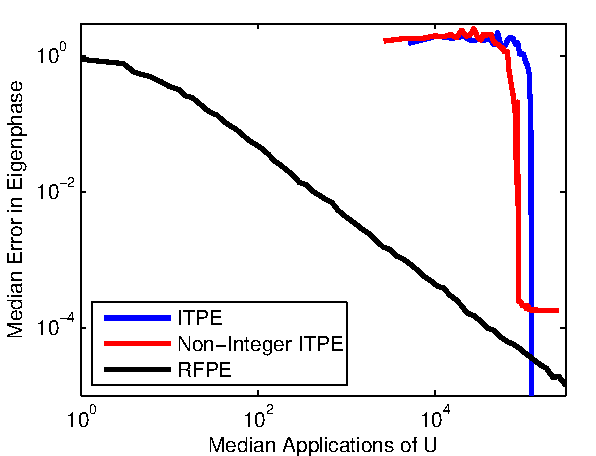
\includegraphics[width=0.723\linewidth]{ITPEcmp.pdf}
    \end{centering}
    \caption{\label{fig:ITPEcmp}
     Comparison of RFPE to ITPE for $t=10~000$ with $100$ samples for $\phi_{\rm true} = 2\pi k/t$ at each measurement.  
    }
\end{figure}



\begin{figure*}
    \begin{centering}
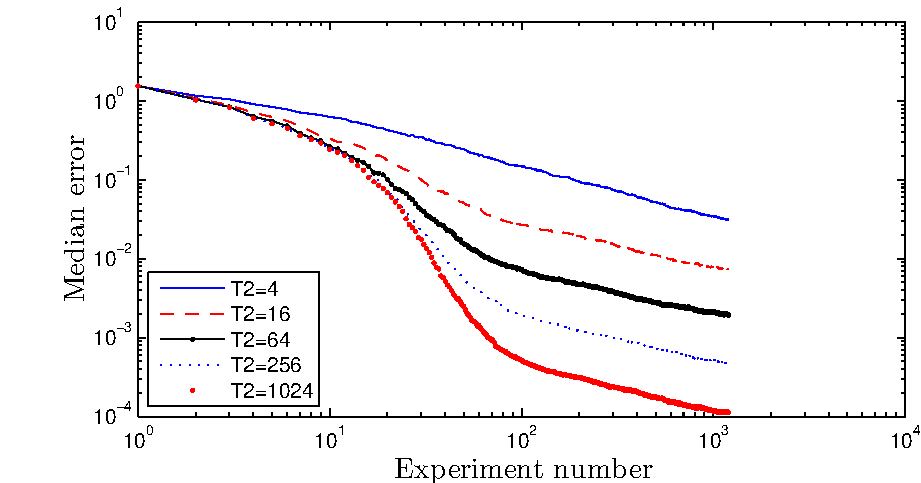
\includegraphics[width=0.45\linewidth]{T2plot_full.pdf}
        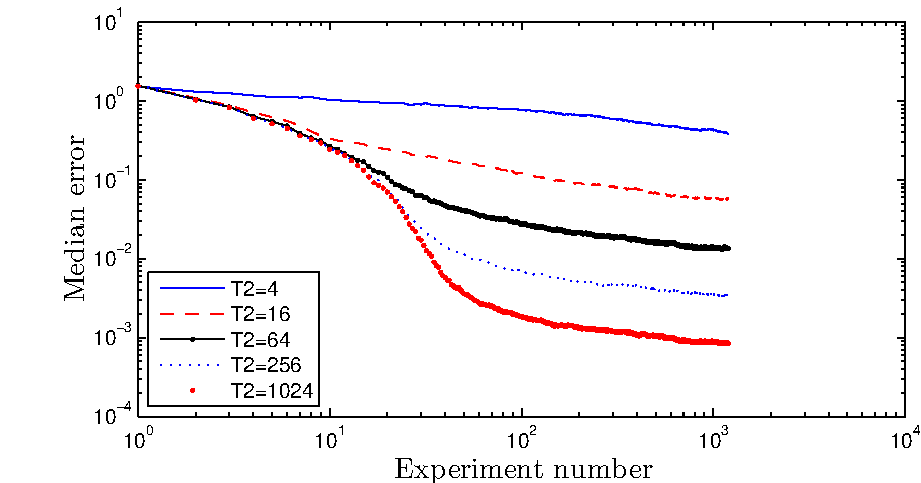
\includegraphics[width=0.45\linewidth]{T2plot.pdf}
    \end{centering}
    \caption{\label{fig:T2plot}
Median errors for phase estimation in decohering systems for experiments constrained to use $M\le T_2$ (left) and $M\le T_2/10$ (right).  We take $m=12~000$, use $1~000$ random samples and take the initial state  to be a random eigenstate.
    }
\end{figure*}

\fig{PEerror} shows the error incurred using RFPE.  The most obvious feature is that the error shrinks exponentially with the number of experiments (which is proportional to the evolution time under the PGH) for $m>100$.  Roughly $150$ experiments are needed for the method to provide $32$ bits of accuracy in the median case.
We discuss the scaling of the mean in the supplemental material.

The number of experiments needed to reach error $\epsilon$ empirically scales as $O(\log(1/\epsilon))$ rather than the $O(\log(1/\epsilon)\log\log(1/\epsilon))$ scaling of Kitaev's method~\cite{Kit96,kitaev2002classical}.  Concretely, after $150$ experiments the median error for Kitaev's PE algorithm (with $s=10$) is roughly $10$ million times that of RFPE.

Although the number of experiments needed is small, the experimental time need
not be.  If the error shrinks as $\epsilon\in \Theta(\ee^{-\lambda N})$ where
$N$ is the experiment number then $T_{\exp}\in O(\sum_{N=1}^{N_{\max}} \ee^{\lambda N})\in O(\ee^{\lambda N_{\rm max}})\in O(1/\epsilon)$.  The
time required saturates the Cram\'er-Rao bound, up to a multiplicative constant.
Specifically, $\lambda\approx 0.17$ for RFPE.

\fig{ITPEcmp} compares our method to information-theory PE (ITPE).  Although it is not adaptive, it is exact and so it is a natural benchmark for comparison.  We find ITPE requires nearly five times the applications of $U$ if $\phi=2\pi k/t$ for integer $k<t$ and $t=10~000$.  

Conversely, ITPE requires only $25$ measurements to identify the phase with $50\%$
probability whereas RFPE requires $51$ experiments if $k$ is an integer.  If
the true value of $k$ is real-valued, then ITPE as stated
fails to learn in the median because the long evolution times chosen lead to
contradictory possibilities that cause ITPE to fail.  We correct
this by choosing $M\rightarrow \lceil M/2\rceil$ in such cases, which increases the number
of experiments to $35$ but also reduces the experimental time below that of
unmodified ITPE.  This shows that all three methods
tradeoff experimental and computational resources differently.

\begin{figure*}
    \begin{centering}
        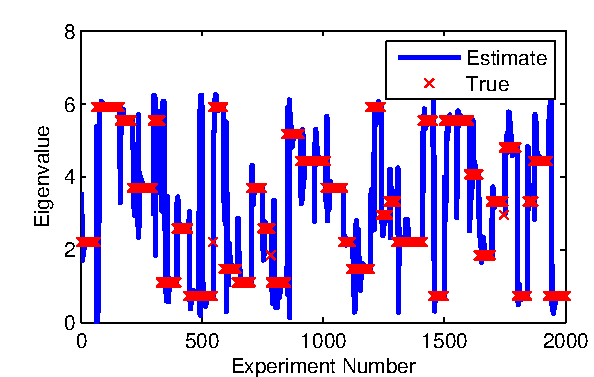
\includegraphics[width=0.4\linewidth]{Errtrack1.pdf}
        \hspace{5mm}
        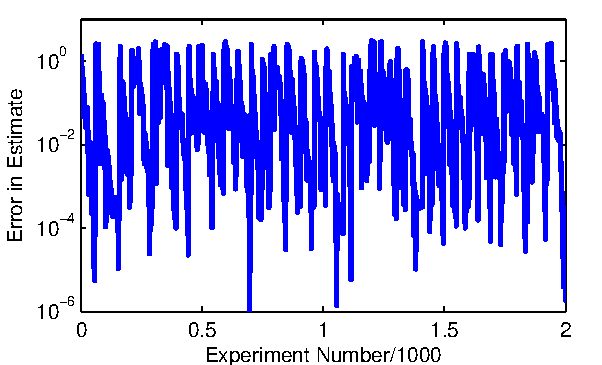
\includegraphics[width=0.4\linewidth]{Errtrack2.pdf}
    \end{centering}
    \caption{\label{fig:Errplot}
        Instantaneous estimate of the eigenphase  for a system with $16$ eigenvalues, $\Delta=0$, $\tau=0.1$ and $T_2=10^4$.
    }
\end{figure*}

%-----------------------------------------------------------------------------
% \subsection{Phase estimation with depolarizing noise}
%-----------------------------------------------------------------------------

A recent criticism of PE methods is that they can be impractical to execute on non--fault tolerant quantum hardware~\cite{PMS+14,MBL+14,WHT15}.  This is because phase estimation attains its quadratic advantage over statistical sampling by using exponentially long evolutions.  Decoherence poses a challenge for these long evolutions because it causes the state to become randomized as time progresses, ultimately resulting in
$\lim_{M\rightarrow \infty} P(0|\phi;\theta,M) = \frac{1}{2}$.
In this limit, the experiments convey no information. 

Decoherence does not place a fundamental limit on the accuracy of PE.   In fact, it has already been observed that Bayesian inference to can be used to learn $\phi$ to an arbitrary number of digits using $M \approx T_2$ for certain noise models~\cite{granade_robust_2012} (at the price of degrading the algorithm's performance).
We investigate the effects of decoherence by assuming the following noise model which is parameterized by the \emph{decoherence time} $T_2$ such that
\begin{gather}
    \label{eq:likedecohere}
    \begin{aligned}
        P(0|\phi) & = \ee^{-M/T_2}\left(\frac{1+\cos(M[\phi -\theta])}{2}\right)+\frac{1-\ee^{-M/T_2}}{2}.
    \end{aligned}
\end{gather}
This model is appropriate when the time required to implement the controlled operation $\Lambda(U)$ is long relative to that required to perform $H$ and an arbitrary $Z$--rotation,
which is in quantum simulation experiments~\cite{hastings2015improving,wecker2015solving,mcclean2014exploiting}.

 

Since $T_2$ constrains the informativeness of long experiments, we propose a variation to \eq{PGH},
\begin{equation}
    \label{eq:pgh2}
    M = \min\left\{\left\lceil\frac{1.25}{\sigma}\right\rceil, T_2 \right\}.
\end{equation}
The experiments yielded by~\eq{pgh2} are qualitatively similar to locally optimized experiments for frequency estimation which are chosen to saturate the Cram\'er-Rao bound \cite{ferrie_how_2013}; however,~\eq{pgh2} requires nearly 100 fold less computing time to select an experiment.
We choose $M$ to cut off at $T_2$ in part because the locally optimized solutions choose to saturate at this value. Indeed, the Cram\'er-Rao bound for frequency estimation scales as $O(M^{-2})$~\cite{WGC15} in the absence of decoherence.  Eqn.~\eq{likedecohere} suggests that decoherence causes the posterior variance to increase as $O(\exp(2M/T_2))$.  Similar to the frequency estimation case \cite{ferrie_how_2013}, $M=T_2$ optimally trades off these tendencies, justifying~\eq{pgh2}.

\fig{T2plot} shows that RFPE smoothly transitions between the exponential scaling expected at short times and the polynomial scaling expected when decoherence becomes significant.  The error scales roughly as $1/N^{0.6}$ in this polynomial regime, which is comparable to the $1/\sqrt{N}$ scaling expected from statistical sampling.  Decoherence therefore does not necessarily fundamentally limit the accuracy that PE can achieve.  \fig{T2plot} also shows that confining the experiments to stay in a more coherent regime also can actually hurt the algorithm's ability to infer the phase, as expected.

%=============================================================================
% \section{Dealing With Noise and Non--Eigenstate Preparations}
% \label{sec:track}
%=============================================================================

In generating \fig{T2plot}, however, we have assumed that the initial quantum state is an eigenstate and is discarded after each experiment. Performing phase estimation in this way minimizes the number of experiments, but can be prohibitively expensive if preparation of the initial eigenstate is prohibitively costly.  

We combat this by retaining the quantum state until it is clear that
a fault has occurred.  Such faults can either be from decoherence or from stochastic errors introduced by rejection filtering.  They
 can cause RFPE to fail because the new data that comes in is only consistent with hypotheses that have been ruled out.
We address this by performing inexpensive experiments to assess whether the state has depolarized or the inference method has failed
and then restart the learning process accordingly.
This reset rule also stabilizes the algorithm when the input state is a superposition of eigenvectors, which underscores its value
even when $T_2=\infty$ (see supplemental material).

The following procedure addresses this issue in cases where the spectral gaps are promised to be at least $\Delta$.
\begin{enumerate}
\item After each update with probability $\ee^{-M/T_2}$ perform an experiment with $\theta=\mu$ and $M=\tau/\sigma$ for $\tau< 1$.
\item If result $=1$ then prepare initial state and reset $\sigma$.
\item After restart, continue as normal until $\sigma<\Delta$ then set $\sigma$ and $\mu$ to those of the closest eigenvalue.
\end{enumerate}

Steps 1 and 2 perform a one--sided test of whether the prior distribution is consistent with the current state.
If the prior probability distribution is correct then the probability of measuring $0$ is
\begin{equation}
    \frac{1}{\sigma\sqrt{2\pi}}\int_{-\infty}^\infty \cos^2\left(\frac{(\mu-x)\tau}{2\sigma}\right)\ee^{-\frac{(\mu-x)^2}{2\sigma^2}} \mathrm{d}x = \frac{1+\ee^{-\tau^2/2}}{2}.
\end{equation}
If $\tau=0.1$, the probability of measuring $0$ is approximately $0.998$ and hence measuring $1$ implies that the hypothesis that the prior is correct can be rejected at $p \le 0.002$. A Bayesian analysis of our reset rule
is given in the supplemental material.

Step 3 restarts the learning process if a fault is detected. It is however important to retain the spectral information that has been learned prior to the restart.  Step 3 reflects this by checking to see if the current estimate of the eigenphase corresponds to a known eigenspace and then sets $\mu$ to be the estimate of the eigenphase and $\sigma$ to be its uncertainty if such an identification is made.  This allows the algorithm to resume learning once the depolarized state is projected onto a known eigenspace.

The test process also permits the eigenvalue of an eigenstate in a decohering system to be estimated in real time. \fig{Errplot} shows that the restarting algorithm can rapidly detect a transition away from an instantaneous eigenstate and then begin inferring the eigenvalue of the system's new instantaneous eigenstate.  This illustrates the stability of RFPE even in the presence of substantial depolarizing noise, thereby addressing many of the critiques of phase estimation.

%=============================================================================
% \section{Conclusion}
%=============================================================================

Our work makes phase estimation more
experimentally relevant by reducing the
experimental time required and by making the process resilient
to decoherence. This is especially critical as current experiments push past the classical
regime and IPE becomes increasingly impractical in lieu of fault-tolerance.
In particular, of our algorithm learns in the presence of decoherence, providing an efficient alternative to the
variational eigensolvers used in present day experiments~\cite{PMS+14,MBL+14,WHT15}.  

Looking at the problem of phase estimation more generally, it is clear that it is in essence an inference problem.
Our work shows that modern ideas from machine learning can be used therein to great effect.  
It is our firm belief that by combining the tools of data science with clever experimental design,
further improvements can be seen not only in phase estimation but also quantum metrology in general.

\acknowledgments{We thank B. Terhal, K. Rudinger and D. Wecker for useful comments.}

%merlin.mbs apsrev4-1.bst 2010-07-25 4.21a (PWD, AO, DPC) hacked
%Control: key (0)
%Control: author (8) initials jnrlst
%Control: editor formatted (1) identically to author
%Control: production of article title (-1) disabled
%Control: page (0) single
%Control: year (1) truncated
%Control: production of eprint (0) enabled
\begin{thebibliography}{31}%
\makeatletter
\providecommand \@ifxundefined [1]{%
 \@ifx{#1\undefined}
}%
\providecommand \@ifnum [1]{%
 \ifnum #1\expandafter \@firstoftwo
 \else \expandafter \@secondoftwo
 \fi
}%
\providecommand \@ifx [1]{%
 \ifx #1\expandafter \@firstoftwo
 \else \expandafter \@secondoftwo
 \fi
}%
\providecommand \natexlab [1]{#1}%
\providecommand \enquote  [1]{``#1''}%
\providecommand \bibnamefont  [1]{#1}%
\providecommand \bibfnamefont [1]{#1}%
\providecommand \citenamefont [1]{#1}%
\providecommand \href@noop [0]{\@secondoftwo}%
\providecommand \href [0]{\begingroup \@sanitize@url \@href}%
\providecommand \@href[1]{\@@startlink{#1}\@@href}%
\providecommand \@@href[1]{\endgroup#1\@@endlink}%
\providecommand \@sanitize@url [0]{\catcode `\\12\catcode `\$12\catcode
  `\&12\catcode `\#12\catcode `\^12\catcode `\_12\catcode `\%12\relax}%
\providecommand \@@startlink[1]{}%
\providecommand \@@endlink[0]{}%
\providecommand \url  [0]{\begingroup\@sanitize@url \@url }%
\providecommand \@url [1]{\endgroup\@href {#1}{\urlprefix }}%
\providecommand \urlprefix  [0]{URL }%
\providecommand \Eprint [0]{\href }%
\providecommand \doibase [0]{http://dx.doi.org/}%
\providecommand \selectlanguage [0]{\@gobble}%
\providecommand \bibinfo  [0]{\@secondoftwo}%
\providecommand \bibfield  [0]{\@secondoftwo}%
\providecommand \translation [1]{[#1]}%
\providecommand \BibitemOpen [0]{}%
\providecommand \bibitemStop [0]{}%
\providecommand \bibitemNoStop [0]{.\EOS\space}%
\providecommand \EOS [0]{\spacefactor3000\relax}%
\providecommand \BibitemShut  [1]{\csname bibitem#1\endcsname}%
\let\auto@bib@innerbib\@empty
%</preamble>
\bibitem [{\citenamefont {Shor}(1997)}]{shor_polynomial-time_1995}%
  \BibitemOpen
  \bibfield  {author} {\bibinfo {author} {\bibfnamefont {P.~W.}\ \bibnamefont
  {Shor}},\ }\href {\doibase 10.1137/S0097539795293172} {\bibfield  {journal}
  {\bibinfo  {journal} {SIAM Journal on Computing}\ }\textbf {\bibinfo {volume}
  {26}},\ \bibinfo {pages} {1484} (\bibinfo {year} {1997})}\BibitemShut
  {NoStop}%
\bibitem [{\citenamefont {Brassard}\ \emph {et~al.}(2002)\citenamefont
  {Brassard}, \citenamefont {Hoyer}, \citenamefont {Mosca},\ and\ \citenamefont
  {Tapp}}]{BHM+02}%
  \BibitemOpen
  \bibfield  {author} {\bibinfo {author} {\bibfnamefont {G.}~\bibnamefont
  {Brassard}}, \bibinfo {author} {\bibfnamefont {P.}~\bibnamefont {Hoyer}},
  \bibinfo {author} {\bibfnamefont {M.}~\bibnamefont {Mosca}}, \ and\ \bibinfo
  {author} {\bibfnamefont {A.}~\bibnamefont {Tapp}},\ }\href {\doibase
  10.1090/conm/305} {\bibfield  {journal} {\bibinfo  {journal} {Contemporary
  Mathematics}\ }\textbf {\bibinfo {volume} {305}},\ \bibinfo {pages} {53}
  (\bibinfo {year} {2002})},\ \Eprint {http://arxiv.org/abs/quant-ph/0005055}
  {quant-ph/0005055} \BibitemShut {NoStop}%
\bibitem [{\citenamefont {Aspuru-Guzik}\ \emph {et~al.}(2005)\citenamefont
  {Aspuru-Guzik}, \citenamefont {Dutoi}, \citenamefont {Love},\ and\
  \citenamefont {Head-Gordon}}]{ADL+05}%
  \BibitemOpen
  \bibfield  {author} {\bibinfo {author} {\bibfnamefont {A.}~\bibnamefont
  {Aspuru-Guzik}}, \bibinfo {author} {\bibfnamefont {A.~D.}\ \bibnamefont
  {Dutoi}}, \bibinfo {author} {\bibfnamefont {P.~J.}\ \bibnamefont {Love}}, \
  and\ \bibinfo {author} {\bibfnamefont {M.}~\bibnamefont {Head-Gordon}},\
  }\href {\doibase 10.1126/science.1113479} {\bibfield  {journal} {\bibinfo
  {journal} {Science}\ }\textbf {\bibinfo {volume} {309}},\ \bibinfo {pages}
  {1704} (\bibinfo {year} {2005})}\BibitemShut {NoStop}%
\bibitem [{\citenamefont {Harrow}\ \emph {et~al.}(2009)\citenamefont {Harrow},
  \citenamefont {Hassidim},\ and\ \citenamefont {Lloyd}}]{harrow2009quantum}%
  \BibitemOpen
  \bibfield  {author} {\bibinfo {author} {\bibfnamefont {A.~W.}\ \bibnamefont
  {Harrow}}, \bibinfo {author} {\bibfnamefont {A.}~\bibnamefont {Hassidim}}, \
  and\ \bibinfo {author} {\bibfnamefont {S.}~\bibnamefont {Lloyd}},\ }\href
  {\doibase 10.1103/PhysRevLett.103.150502} {\bibfield  {journal} {\bibinfo
  {journal} {Physical Review Letters}\ }\textbf {\bibinfo {volume} {103}},\
  \bibinfo {pages} {150502} (\bibinfo {year} {2009})}\BibitemShut {NoStop}%
\bibitem [{\citenamefont {Lanyon}\ \emph {et~al.}(2010)\citenamefont {Lanyon},
  \citenamefont {Whitfield}, \citenamefont {Gillett}, \citenamefont {Goggin},
  \citenamefont {Almeida}, \citenamefont {Kassal}, \citenamefont {Biamonte},
  \citenamefont {Mohseni}, \citenamefont {Powell}, \citenamefont {Barbieri}
  \emph {et~al.}}]{lanyon2010towards}%
  \BibitemOpen
  \bibfield  {author} {\bibinfo {author} {\bibfnamefont {B.~P.}\ \bibnamefont
  {Lanyon}}, \bibinfo {author} {\bibfnamefont {J.~D.}\ \bibnamefont
  {Whitfield}}, \bibinfo {author} {\bibfnamefont {G.}~\bibnamefont {Gillett}},
  \bibinfo {author} {\bibfnamefont {M.~E.}\ \bibnamefont {Goggin}}, \bibinfo
  {author} {\bibfnamefont {M.~P.}\ \bibnamefont {Almeida}}, \bibinfo {author}
  {\bibfnamefont {I.}~\bibnamefont {Kassal}}, \bibinfo {author} {\bibfnamefont
  {J.~D.}\ \bibnamefont {Biamonte}}, \bibinfo {author} {\bibfnamefont
  {M.}~\bibnamefont {Mohseni}}, \bibinfo {author} {\bibfnamefont {B.~J.}\
  \bibnamefont {Powell}}, \bibinfo {author} {\bibfnamefont {M.}~\bibnamefont
  {Barbieri}},  \emph {et~al.},\ }\href {\doibase 10.1038/nchem.483} {\bibfield
   {journal} {\bibinfo  {journal} {Nature Chemistry}\ }\textbf {\bibinfo
  {volume} {2}},\ \bibinfo {pages} {106} (\bibinfo {year} {2010})}\BibitemShut
  {NoStop}%
\bibitem [{\citenamefont {Kitaev}(1996)}]{Kit96}%
  \BibitemOpen
  \bibfield  {author} {\bibinfo {author} {\bibfnamefont {A.~Y.}\ \bibnamefont
  {Kitaev}},\ }\href {http://eccc.hpi-web.de/report/1996/003/} {\bibfield
  {journal} {\bibinfo  {journal} {Electronic Colloquium on Computational
  Complexity}\ }\textbf {\bibinfo {volume} {3}} (\bibinfo {year}
  {1996})}\BibitemShut {NoStop}%
\bibitem [{\citenamefont {Kitaev}\ \emph {et~al.}(2002)\citenamefont {Kitaev},
  \citenamefont {Shen},\ and\ \citenamefont {Vyalyi}}]{kitaev2002classical}%
  \BibitemOpen
  \bibfield  {author} {\bibinfo {author} {\bibfnamefont {A.~Y.}\ \bibnamefont
  {Kitaev}}, \bibinfo {author} {\bibfnamefont {A.}~\bibnamefont {Shen}}, \ and\
  \bibinfo {author} {\bibfnamefont {M.~N.}\ \bibnamefont {Vyalyi}},\
  }\href@noop {} {\emph {\bibinfo {title} {Classical and quantum
  computation}}},\ Vol.~\bibinfo {volume} {47}\ (\bibinfo  {publisher}
  {American Mathematical Society Providence},\ \bibinfo {year}
  {2002})\BibitemShut {NoStop}%
\bibitem [{\citenamefont {Higgins}\ \emph {et~al.}(2007)\citenamefont
  {Higgins}, \citenamefont {Berry}, \citenamefont {Bartlett}, \citenamefont
  {Wiseman},\ and\ \citenamefont {Pryde}}]{higgins2007entanglement}%
  \BibitemOpen
  \bibfield  {author} {\bibinfo {author} {\bibfnamefont {B.~L.}\ \bibnamefont
  {Higgins}}, \bibinfo {author} {\bibfnamefont {D.~W.}\ \bibnamefont {Berry}},
  \bibinfo {author} {\bibfnamefont {S.~D.}\ \bibnamefont {Bartlett}}, \bibinfo
  {author} {\bibfnamefont {H.~M.}\ \bibnamefont {Wiseman}}, \ and\ \bibinfo
  {author} {\bibfnamefont {G.~J.}\ \bibnamefont {Pryde}},\ }\href {\doibase
  10.1038/nature06257} {\bibfield  {journal} {\bibinfo  {journal} {Nature}\
  }\textbf {\bibinfo {volume} {450}},\ \bibinfo {pages} {393} (\bibinfo {year}
  {2007})}\BibitemShut {NoStop}%
\bibitem [{\citenamefont {Svore}\ \emph {et~al.}(2014)\citenamefont {Svore},
  \citenamefont {Hastings},\ and\ \citenamefont {Freedman}}]{SHF14}%
  \BibitemOpen
  \bibfield  {author} {\bibinfo {author} {\bibfnamefont {K.~M.}\ \bibnamefont
  {Svore}}, \bibinfo {author} {\bibfnamefont {M.~B.}\ \bibnamefont {Hastings}},
  \ and\ \bibinfo {author} {\bibfnamefont {M.}~\bibnamefont {Freedman}},\
  }\href@noop {} {\bibfield  {journal} {\bibinfo  {journal} {Quantum
  Information \& Computation}\ }\textbf {\bibinfo {volume} {14}},\ \bibinfo
  {pages} {306} (\bibinfo {year} {2014})}\BibitemShut {NoStop}%
\bibitem [{\citenamefont {Kimmel}\ \emph {et~al.}(2015)\citenamefont {Kimmel},
  \citenamefont {Low},\ and\ \citenamefont {Yoder}}]{KLY15}%
  \BibitemOpen
  \bibfield  {author} {\bibinfo {author} {\bibfnamefont {S.}~\bibnamefont
  {Kimmel}}, \bibinfo {author} {\bibfnamefont {G.~H.}\ \bibnamefont {Low}}, \
  and\ \bibinfo {author} {\bibfnamefont {T.~J.}\ \bibnamefont {Yoder}},\
  }\href@noop {} {\bibfield  {journal} {\bibinfo  {journal} {arXiv preprint
  arXiv:1502.02677}\ } (\bibinfo {year} {2015})}\BibitemShut {NoStop}%
\bibitem [{\citenamefont {Granade}\ \emph {et~al.}(2012)\citenamefont
  {Granade}, \citenamefont {Ferrie}, \citenamefont {Wiebe},\ and\ \citenamefont
  {Cory}}]{granade_robust_2012}%
  \BibitemOpen
  \bibfield  {author} {\bibinfo {author} {\bibfnamefont {C.~E.}\ \bibnamefont
  {Granade}}, \bibinfo {author} {\bibfnamefont {C.}~\bibnamefont {Ferrie}},
  \bibinfo {author} {\bibfnamefont {N.}~\bibnamefont {Wiebe}}, \ and\ \bibinfo
  {author} {\bibfnamefont {D.~G.}\ \bibnamefont {Cory}},\ }\href {\doibase
  10.1088/1367-2630/14/10/103013} {\bibfield  {journal} {\bibinfo  {journal}
  {New Journal of Physics}\ }\textbf {\bibinfo {volume} {14}},\ \bibinfo
  {pages} {103013} (\bibinfo {year} {2012})}\BibitemShut {NoStop}%
\bibitem [{\citenamefont {Ferrie}(2014)}]{ferrie_high_2014}%
  \BibitemOpen
  \bibfield  {author} {\bibinfo {author} {\bibfnamefont {C.}~\bibnamefont
  {Ferrie}},\ }\href {\doibase 10.1088/1367-2630/16/2/023006} {\bibfield
  {journal} {\bibinfo  {journal} {New Journal of Physics}\ }\textbf {\bibinfo
  {volume} {16}},\ \bibinfo {pages} {023006} (\bibinfo {year}
  {2014})}\BibitemShut {NoStop}%
\bibitem [{\citenamefont {Haykin}(2004)}]{haykin2004kalman}%
  \BibitemOpen
  \bibfield  {author} {\bibinfo {author} {\bibfnamefont {S.}~\bibnamefont
  {Haykin}},\ }\href@noop {} {\emph {\bibinfo {title} {Kalman filtering and
  neural networks}}},\ Vol.~\bibinfo {volume} {47}\ (\bibinfo  {publisher}
  {John Wiley \& Sons},\ \bibinfo {year} {2004})\BibitemShut {NoStop}%
\bibitem [{\citenamefont {Smith}\ \emph {et~al.}(2013)\citenamefont {Smith},
  \citenamefont {Doucet}, \citenamefont {de~Freitas},\ and\ \citenamefont
  {Gordon}}]{smith2013sequential}%
  \BibitemOpen
  \bibfield  {author} {\bibinfo {author} {\bibfnamefont {A.}~\bibnamefont
  {Smith}}, \bibinfo {author} {\bibfnamefont {A.}~\bibnamefont {Doucet}},
  \bibinfo {author} {\bibfnamefont {N.}~\bibnamefont {de~Freitas}}, \ and\
  \bibinfo {author} {\bibfnamefont {N.}~\bibnamefont {Gordon}},\ }\href@noop {}
  {\emph {\bibinfo {title} {Sequential Monte Carlo methods in practice}}}\
  (\bibinfo  {publisher} {Springer Science \& Business Media},\ \bibinfo {year}
  {2013})\BibitemShut {NoStop}%
\bibitem [{\citenamefont {Isard}\ and\ \citenamefont
  {Blake}(1998)}]{isard_condensationconditional_1998}%
  \BibitemOpen
  \bibfield  {author} {\bibinfo {author} {\bibfnamefont {M.}~\bibnamefont
  {Isard}}\ and\ \bibinfo {author} {\bibfnamefont {A.}~\bibnamefont {Blake}},\
  }\href {\doibase 10.1023/A:1008078328650} {\bibfield  {journal} {\bibinfo
  {journal} {International Journal of Computer Vision}\ }\textbf {\bibinfo
  {volume} {29}},\ \bibinfo {pages} {5} (\bibinfo {year} {1998})}\BibitemShut
  {NoStop}%
\bibitem [{\citenamefont {Shulman}\ \emph {et~al.}(2014)\citenamefont
  {Shulman}, \citenamefont {Harvey}, \citenamefont {Nichol}, \citenamefont
  {Bartlett}, \citenamefont {Doherty}, \citenamefont {Umansky},\ and\
  \citenamefont {Yacoby}}]{shulman_suppressing_2014}%
  \BibitemOpen
  \bibfield  {author} {\bibinfo {author} {\bibfnamefont {M.~D.}\ \bibnamefont
  {Shulman}}, \bibinfo {author} {\bibfnamefont {S.~P.}\ \bibnamefont {Harvey}},
  \bibinfo {author} {\bibfnamefont {J.~M.}\ \bibnamefont {Nichol}}, \bibinfo
  {author} {\bibfnamefont {S.~D.}\ \bibnamefont {Bartlett}}, \bibinfo {author}
  {\bibfnamefont {A.~C.}\ \bibnamefont {Doherty}}, \bibinfo {author}
  {\bibfnamefont {V.}~\bibnamefont {Umansky}}, \ and\ \bibinfo {author}
  {\bibfnamefont {A.}~\bibnamefont {Yacoby}},\ }\href {\doibase
  10.1038/ncomms6156} {\bibfield  {journal} {\bibinfo  {journal} {Nature
  Communications}\ }\textbf {\bibinfo {volume} {5}},\ \bibinfo {pages} {5156}
  (\bibinfo {year} {2014})}\BibitemShut {NoStop}%
\bibitem [{\citenamefont {Casagrande}(2014)}]{casagrande_design_2014}%
  \BibitemOpen
  \bibfield  {author} {\bibinfo {author} {\bibfnamefont {S.}~\bibnamefont
  {Casagrande}},\ }\href {https://uwspace.uwaterloo.ca/handle/10012/8281}
  {\enquote {\bibinfo {title} {On design and testing of a spectrometer based on
  an {FPGA} development board for use with optimal control theory and high-{Q}
  resonators},}\ } (\bibinfo {year} {2014})\BibitemShut {NoStop}%
\bibitem [{\citenamefont {Hornibrook}\ \emph {et~al.}(2015)\citenamefont
  {Hornibrook}, \citenamefont {Colless}, \citenamefont {Conway~Lamb},
  \citenamefont {Pauka}, \citenamefont {Lu}, \citenamefont {Gossard},
  \citenamefont {Watson}, \citenamefont {Gardner}, \citenamefont {Fallahi},
  \citenamefont {Manfra},\ and\ \citenamefont
  {Reilly}}]{hornibrook_cryogenic_2015}%
  \BibitemOpen
  \bibfield  {author} {\bibinfo {author} {\bibfnamefont {J.}~\bibnamefont
  {Hornibrook}}, \bibinfo {author} {\bibfnamefont {J.}~\bibnamefont {Colless}},
  \bibinfo {author} {\bibfnamefont {I.}~\bibnamefont {Conway~Lamb}}, \bibinfo
  {author} {\bibfnamefont {S.}~\bibnamefont {Pauka}}, \bibinfo {author}
  {\bibfnamefont {H.}~\bibnamefont {Lu}}, \bibinfo {author} {\bibfnamefont
  {A.}~\bibnamefont {Gossard}}, \bibinfo {author} {\bibfnamefont
  {J.}~\bibnamefont {Watson}}, \bibinfo {author} {\bibfnamefont
  {G.}~\bibnamefont {Gardner}}, \bibinfo {author} {\bibfnamefont
  {S.}~\bibnamefont {Fallahi}}, \bibinfo {author} {\bibfnamefont
  {M.}~\bibnamefont {Manfra}}, \ and\ \bibinfo {author} {\bibfnamefont
  {D.}~\bibnamefont {Reilly}},\ }\href {\doibase
  10.1103/PhysRevApplied.3.024010} {\bibfield  {journal} {\bibinfo  {journal}
  {Physical Review Applied}\ }\textbf {\bibinfo {volume} {3}},\ \bibinfo
  {pages} {024010} (\bibinfo {year} {2015})}\BibitemShut {NoStop}%
\bibitem [{\citenamefont {Opper}\ and\ \citenamefont
  {Winther}(1998)}]{opper1998bayesian}%
  \BibitemOpen
  \bibfield  {author} {\bibinfo {author} {\bibfnamefont {M.}~\bibnamefont
  {Opper}}\ and\ \bibinfo {author} {\bibfnamefont {O.}~\bibnamefont
  {Winther}},\ }\href {http://dl.acm.org/citation.cfm?id=304710.304756}
  {\bibfield  {journal} {\bibinfo  {journal} {On-line Learning in Neural
  Networks}\ ,\ \bibinfo {pages} {363}} (\bibinfo {year} {1998})}\BibitemShut
  {NoStop}%
\bibitem [{\citenamefont {Wiebe}\ \emph
  {et~al.}(2014{\natexlab{a}})\citenamefont {Wiebe}, \citenamefont {Granade},
  \citenamefont {Ferrie},\ and\ \citenamefont {Cory}}]{wiebe_hamiltonian_2014}%
  \BibitemOpen
  \bibfield  {author} {\bibinfo {author} {\bibfnamefont {N.}~\bibnamefont
  {Wiebe}}, \bibinfo {author} {\bibfnamefont {C.}~\bibnamefont {Granade}},
  \bibinfo {author} {\bibfnamefont {C.}~\bibnamefont {Ferrie}}, \ and\ \bibinfo
  {author} {\bibfnamefont {D.}~\bibnamefont {Cory}},\ }\href {\doibase
  10.1103/PhysRevLett.112.190501} {\bibfield  {journal} {\bibinfo  {journal}
  {Physical Review Letters}\ }\textbf {\bibinfo {volume} {112}},\ \bibinfo
  {pages} {190501} (\bibinfo {year} {2014}{\natexlab{a}})}\BibitemShut
  {NoStop}%
\bibitem [{\citenamefont {Peruzzo}\ \emph {et~al.}(2014)\citenamefont
  {Peruzzo}, \citenamefont {McClean}, \citenamefont {Shadbolt}, \citenamefont
  {Yung}, \citenamefont {Zhou}, \citenamefont {Love}, \citenamefont
  {Aspuru-Guzik},\ and\ \citenamefont {O’Brien}}]{PMS+14}%
  \BibitemOpen
  \bibfield  {author} {\bibinfo {author} {\bibfnamefont {A.}~\bibnamefont
  {Peruzzo}}, \bibinfo {author} {\bibfnamefont {J.}~\bibnamefont {McClean}},
  \bibinfo {author} {\bibfnamefont {P.}~\bibnamefont {Shadbolt}}, \bibinfo
  {author} {\bibfnamefont {M.-H.}\ \bibnamefont {Yung}}, \bibinfo {author}
  {\bibfnamefont {X.-Q.}\ \bibnamefont {Zhou}}, \bibinfo {author}
  {\bibfnamefont {P.~J.}\ \bibnamefont {Love}}, \bibinfo {author}
  {\bibfnamefont {A.}~\bibnamefont {Aspuru-Guzik}}, \ and\ \bibinfo {author}
  {\bibfnamefont {J.~L.}\ \bibnamefont {O’Brien}},\ }\href {\doibase
  10.1038/ncomms5213} {\bibfield  {journal} {\bibinfo  {journal} {Nature
  Communications}\ }\textbf {\bibinfo {volume} {5}},\ \bibinfo {pages} {4213}
  (\bibinfo {year} {2014})}\BibitemShut {NoStop}%
\bibitem [{\citenamefont {McClean}\ \emph
  {et~al.}(2014{\natexlab{a}})\citenamefont {McClean}, \citenamefont {Babbush},
  \citenamefont {Love},\ and\ \citenamefont {Aspuru-Guzik}}]{MBL+14}%
  \BibitemOpen
  \bibfield  {author} {\bibinfo {author} {\bibfnamefont {J.~R.}\ \bibnamefont
  {McClean}}, \bibinfo {author} {\bibfnamefont {R.}~\bibnamefont {Babbush}},
  \bibinfo {author} {\bibfnamefont {P.~J.}\ \bibnamefont {Love}}, \ and\
  \bibinfo {author} {\bibfnamefont {A.}~\bibnamefont {Aspuru-Guzik}},\ }\href
  {\doibase 10.1021/jz501649m} {\bibfield  {journal} {\bibinfo  {journal}
  {Journal of Physical Chemistry Letters}\ }\textbf {\bibinfo {volume} {5}},\
  \bibinfo {pages} {4368} (\bibinfo {year} {2014}{\natexlab{a}})}\BibitemShut
  {NoStop}%
\bibitem [{\citenamefont {Wecker}\ \emph
  {et~al.}(2015{\natexlab{a}})\citenamefont {Wecker}, \citenamefont
  {Hastings},\ and\ \citenamefont {Troyer}}]{WHT15}%
  \BibitemOpen
  \bibfield  {author} {\bibinfo {author} {\bibfnamefont {D.}~\bibnamefont
  {Wecker}}, \bibinfo {author} {\bibfnamefont {M.}~\bibnamefont {Hastings}}, \
  and\ \bibinfo {author} {\bibfnamefont {M.}~\bibnamefont {Troyer}},\
  }\href@noop {} {\bibfield  {journal} {\bibinfo  {journal}
  {arXiv:1507.08969v1}\ } (\bibinfo {year} {2015}{\natexlab{a}})}\BibitemShut
  {NoStop}%
\bibitem [{\citenamefont {Hastings}\ \emph {et~al.}(2015)\citenamefont
  {Hastings}, \citenamefont {Wecker}, \citenamefont {Bauer},\ and\
  \citenamefont {Troyer}}]{hastings2015improving}%
  \BibitemOpen
  \bibfield  {author} {\bibinfo {author} {\bibfnamefont {M.~B.}\ \bibnamefont
  {Hastings}}, \bibinfo {author} {\bibfnamefont {D.}~\bibnamefont {Wecker}},
  \bibinfo {author} {\bibfnamefont {B.}~\bibnamefont {Bauer}}, \ and\ \bibinfo
  {author} {\bibfnamefont {M.}~\bibnamefont {Troyer}},\ }\href@noop {}
  {\bibfield  {journal} {\bibinfo  {journal} {Quantum Information \&
  Computation}\ }\textbf {\bibinfo {volume} {15}},\ \bibinfo {pages} {1}
  (\bibinfo {year} {2015})}\BibitemShut {NoStop}%
\bibitem [{\citenamefont {Wecker}\ \emph
  {et~al.}(2015{\natexlab{b}})\citenamefont {Wecker}, \citenamefont {Hastings},
  \citenamefont {Wiebe}, \citenamefont {Clark}, \citenamefont {Nayak},\ and\
  \citenamefont {Troyer}}]{wecker2015solving}%
  \BibitemOpen
  \bibfield  {author} {\bibinfo {author} {\bibfnamefont {D.}~\bibnamefont
  {Wecker}}, \bibinfo {author} {\bibfnamefont {M.~B.}\ \bibnamefont
  {Hastings}}, \bibinfo {author} {\bibfnamefont {N.}~\bibnamefont {Wiebe}},
  \bibinfo {author} {\bibfnamefont {B.~K.}\ \bibnamefont {Clark}}, \bibinfo
  {author} {\bibfnamefont {C.}~\bibnamefont {Nayak}}, \ and\ \bibinfo {author}
  {\bibfnamefont {M.}~\bibnamefont {Troyer}},\ }\href@noop {} {\bibfield
  {journal} {\bibinfo  {journal} {arXiv preprint arXiv:1506.05135}\ } (\bibinfo
  {year} {2015}{\natexlab{b}})}\BibitemShut {NoStop}%
\bibitem [{\citenamefont {McClean}\ \emph
  {et~al.}(2014{\natexlab{b}})\citenamefont {McClean}, \citenamefont {Babbush},
  \citenamefont {Love},\ and\ \citenamefont
  {Aspuru-Guzik}}]{mcclean2014exploiting}%
  \BibitemOpen
  \bibfield  {author} {\bibinfo {author} {\bibfnamefont {J.~R.}\ \bibnamefont
  {McClean}}, \bibinfo {author} {\bibfnamefont {R.}~\bibnamefont {Babbush}},
  \bibinfo {author} {\bibfnamefont {P.~J.}\ \bibnamefont {Love}}, \ and\
  \bibinfo {author} {\bibfnamefont {A.}~\bibnamefont {Aspuru-Guzik}},\
  }\href@noop {} {\bibfield  {journal} {\bibinfo  {journal} {The Journal of
  Physical Chemistry Letters}\ }\textbf {\bibinfo {volume} {5}},\ \bibinfo
  {pages} {4368} (\bibinfo {year} {2014}{\natexlab{b}})}\BibitemShut {NoStop}%
\bibitem [{\citenamefont {Ferrie}\ \emph {et~al.}(2013)\citenamefont {Ferrie},
  \citenamefont {Granade},\ and\ \citenamefont {Cory}}]{ferrie_how_2013}%
  \BibitemOpen
  \bibfield  {author} {\bibinfo {author} {\bibfnamefont {C.}~\bibnamefont
  {Ferrie}}, \bibinfo {author} {\bibfnamefont {C.~E.}\ \bibnamefont {Granade}},
  \ and\ \bibinfo {author} {\bibfnamefont {D.~G.}\ \bibnamefont {Cory}},\
  }\href {http://link.springer.com/article/10.1007/s11128-012-0407-6}
  {\bibfield  {journal} {\bibinfo  {journal} {Quantum Information Processing}\
  }\textbf {\bibinfo {volume} {12}},\ \bibinfo {pages} {611} (\bibinfo {year}
  {2013})}\BibitemShut {NoStop}%
\bibitem [{\citenamefont {Wiebe}\ \emph {et~al.}(2015)\citenamefont {Wiebe},
  \citenamefont {Granade},\ and\ \citenamefont {Cory}}]{WGC15}%
  \BibitemOpen
  \bibfield  {author} {\bibinfo {author} {\bibfnamefont {N.}~\bibnamefont
  {Wiebe}}, \bibinfo {author} {\bibfnamefont {C.}~\bibnamefont {Granade}}, \
  and\ \bibinfo {author} {\bibfnamefont {D.~G.}\ \bibnamefont {Cory}},\ }\href
  {\doibase 10.1088/1367-2630/17/2/022005} {\bibfield  {journal} {\bibinfo
  {journal} {New Journal of Physics}\ }\textbf {\bibinfo {volume} {17}},\
  \bibinfo {pages} {022005} (\bibinfo {year} {2015})}\BibitemShut {NoStop}%
\bibitem [{\citenamefont {Wiebe}\ \emph
  {et~al.}(2014{\natexlab{b}})\citenamefont {Wiebe}, \citenamefont {Granade},
  \citenamefont {Ferrie},\ and\ \citenamefont {Cory}}]{wiebe_quantum_2014-1}%
  \BibitemOpen
  \bibfield  {author} {\bibinfo {author} {\bibfnamefont {N.}~\bibnamefont
  {Wiebe}}, \bibinfo {author} {\bibfnamefont {C.}~\bibnamefont {Granade}},
  \bibinfo {author} {\bibfnamefont {C.}~\bibnamefont {Ferrie}}, \ and\ \bibinfo
  {author} {\bibfnamefont {D.}~\bibnamefont {Cory}},\ }\href {\doibase
  10.1103/PhysRevA.89.042314} {\bibfield  {journal} {\bibinfo  {journal}
  {Physical Review A}\ }\textbf {\bibinfo {volume} {89}},\ \bibinfo {pages}
  {042314} (\bibinfo {year} {2014}{\natexlab{b}})}\BibitemShut {NoStop}%
\bibitem [{\citenamefont {Goodman}(2008)}]{goodman_dirty_2008}%
  \BibitemOpen
  \bibfield  {author} {\bibinfo {author} {\bibfnamefont {S.}~\bibnamefont
  {Goodman}},\ }\href {\doibase 10.1053/j.seminhematol.2008.04.003} {\bibfield
  {journal} {\bibinfo  {journal} {Seminars in Hematology}\ }\bibinfo {series}
  {Interpretation of {Quantitative} {Research}},\ \textbf {\bibinfo {volume}
  {45}},\ \bibinfo {pages} {135} (\bibinfo {year} {2008})}\BibitemShut
  {NoStop}%
\bibitem [{\citenamefont {Hoekstra}\ \emph {et~al.}(2014)\citenamefont
  {Hoekstra}, \citenamefont {Morey}, \citenamefont {Rouder},\ and\
  \citenamefont {Wagenmakers}}]{hoekstra_robust_2014}%
  \BibitemOpen
  \bibfield  {author} {\bibinfo {author} {\bibfnamefont {R.}~\bibnamefont
  {Hoekstra}}, \bibinfo {author} {\bibfnamefont {R.~D.}\ \bibnamefont {Morey}},
  \bibinfo {author} {\bibfnamefont {J.~N.}\ \bibnamefont {Rouder}}, \ and\
  \bibinfo {author} {\bibfnamefont {E.-J.}\ \bibnamefont {Wagenmakers}},\
  }\href {\doibase 10.3758/s13423-013-0572-3} {\bibfield  {journal} {\bibinfo
  {journal} {Psychonomic Bulletin \& Review}\ ,\ \bibinfo {pages} {1}}
  (\bibinfo {year} {2014})}\BibitemShut {NoStop}%
\end{thebibliography}%
\end{document}